\section{MuhammadIqbalPanggabean(1174063)}

\subsection{Koordinat}
Koordinat didapatkan dari hasil perpotongan antara garis latitude (Y) / lintang dan garis longitude(X) / garis bujur sehingga bisa menunjukan suatu lokasi pada suatu daerah. \hfill\break 
Umumnya koordinat dibedakan menajadi koordinat Geografi dan Universal Transver Mercator(UTM). Pada koordinat geografi dibedakan menajadi 3 yaitu : \hfill\break
\begin{itemize}
	\item Degree, Decimal(DD, DDDD) contoh S 4.56734 E 102.67235
	\item Degree,Minute(DD MM,MMMM) contoh S 4 42,5423’ E 105 34,6445’
	\item Degree, Minute, Second(DD MM SS,SS) contoh : S 4 43’ 45,22 E 103 33’ 33,25
\end{itemize}
\hfill\break
\begin{figure}[H]
	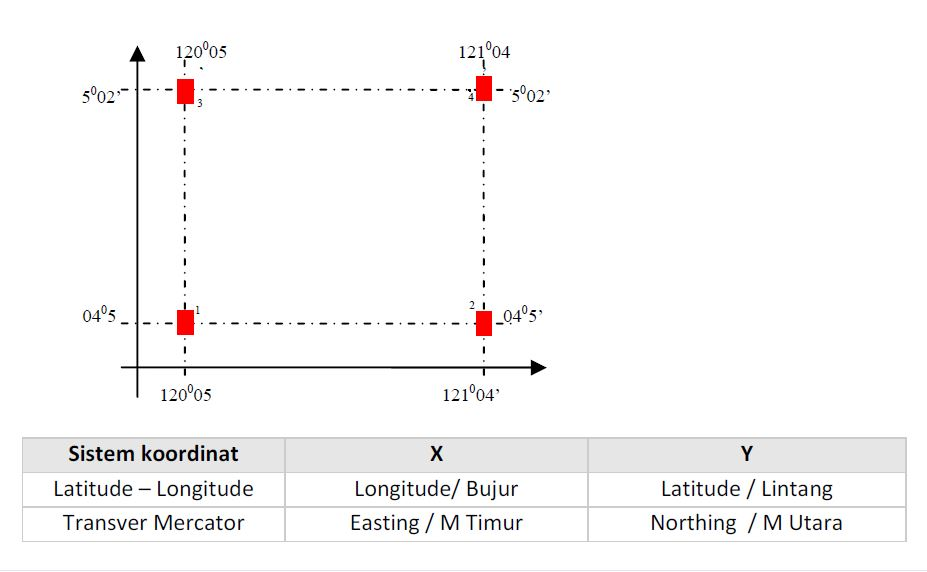
\includegraphics[width=4cm]{figures/1174063/koordinat.jpg}
	\centering
	\caption{Contoh Koordinat}
\end{figure}
Pada system koordinat UTM biasanya terdapat pembagian waktu berdasarkan zonasinya. \hfill\break
\begin{figure}[H]
	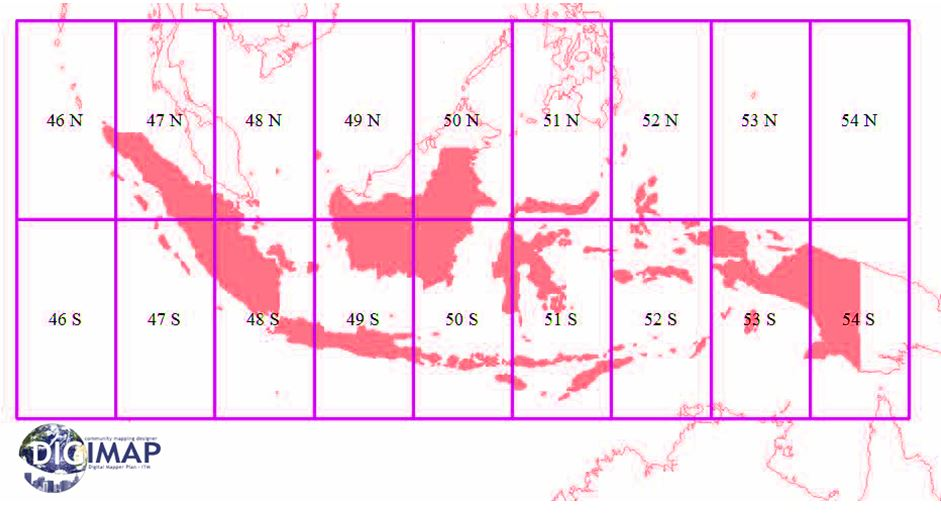
\includegraphics[width=4cm]{figures/1174063/utm.jpg}
	\centering
	\caption{Contoh Koordinat UTM}
\end{figure}

	\subsection{Link}
\href{https://youtu.be/mU4dPSOHDWI}{LOOK AT THIS}
\subsection{Plagiarism}
\begin{figure}[H]
	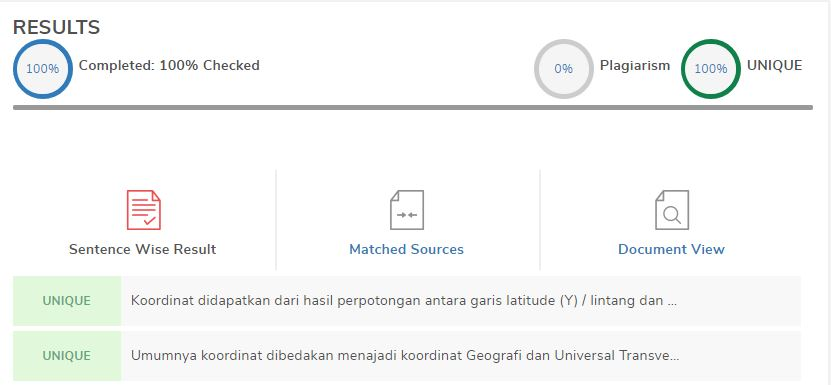
\includegraphics[width=4cm]{figures/1174063/plagiat.jpg}
	\centering
	\caption{Plagiat.}
\end{figure}

